\documentclass[]{beamer}
%\documentclass{article}
%\usepackage{beamerarticle}

\mode<presentation>
{
  \usetheme{Warsaw}
  % or ...

  \setbeamercovered{transparent}
  % or whatever (possibly just delete it)
}


\usepackage[english]{babel}
% or whatever

\usepackage[utf8]{inputenc}
% or whatever

\usepackage{times}
\usepackage[T1]{fontenc}
\usepackage{tikz}
\usetikzlibrary{arrows.meta}

%%%%%%%%%%%%%%%%%%%%%%%%%%%%%%%%%%
%%                         PACKAGES                      %%
%%%%%%%%%%%%%%%%%%%%%%%%%%%%%%%%%%
\usepackage{hyperref,ctable}
\usepackage{graphicx}
\usepackage{tikz}                    % For flowchart
\usetikzlibrary{shapes,arrows} % For flowchart


%%%%%%%%%%%%%%%%%%%%%%%%%%%%%%%%%%
%%                           COLORS                        %%
%%%%%%%%%%%%%%%%%%%%%%%%%%%%%%%%%%
%AU COLORS
\definecolor{aublue}{RGB}{25,33,129}
\definecolor{aured}{RGB}{244,28,31}

%Red
%\setbeamercolor{titlelike}{bg=aured,fg=white}
\setbeamercolor{structure}{bg=black!25!aured, fg=aured}
%\setbeamercolor*{palette primary}{fg=white,bg=aured}
%\setbeamercolor*{palette quaternary}{fg=white,bg=aublue}

%Blue
\setbeamercolor{titlelike}{bg=aublue,fg=white}
%\setbeamercolor{structure}{bg=black!25!aublue, fg=aublue}
\setbeamercolor*{palette primary}{fg=white,bg=aublue}
\setbeamercolor*{palette quaternary}{fg=white,bg=black!75!aublue}

\setbeamercolor{local structure}{fg=aured,bg=gray!60!aured}
\setbeamercolor{alerted text}{fg=aured}

\newenvironment{concept}[1]%
	{
	\setbeamercolor{background canvas}{bg=aured!10!white}%
	\setbeamercolor{frametitle}{bg=aured}%
	\setbeamercolor{frametitle right}{bg=aured}
	\setbeamercolor{alerted text}{fg=aured}%
	\begin{frame}{Concept}%
	\alert{\bfseries \large #1\\[2em]}}{%
	\end{frame}%
	}


%%%%%%%%%%%%%%%%%%%%%%%%%%%%%%%%%%
%%                         GRAPHICS                       %%
%%%%%%%%%%%%%%%%%%%%%%%%%%%%%%%%%%
%\graphicspath{{/Users/bader/work/Presentations/Images/}}}}


%%%%%%%%%%%%%%%%%%%%%%%%%%%%%%%%%%
%%                        COMMANDS                       %%
%%%%%%%%%%%%%%%%%%%%%%%%%%%%%%%%%%
\newcommand{\strong}[1]{\textbf{#1}}
\AtBeginSection[]{
  \begin{frame}
  \vfill
  \centering
  \begin{beamercolorbox}[sep=8pt,center,shadow=true,rounded=true]{title}
    \usebeamerfont{title}\insertsectionhead\par%
  \end{beamercolorbox}
  \vfill
  \end{frame}
}



%%%%%%%%%%%%%%%%%%%%%%%%%%%%%%%%%%
%%                     PRESENTATION                   %%
%%%%%%%%%%%%%%%%%%%%%%%%%%%%%%%%%%
\title[Questions \& Answers]{Questions and Answers in Surveys}

\author[Bader--SOCY 625]
{Michael D.~M.~Bader}

\institute 
{
  Practicum in Sociological Research (SOCY 625)
}
% - Use the \inst command only if there are several affiliations.
% - Keep it simple, no one is interested in your street address.

\date % (optional)
{Week 6}

\subject{Practicum in Sociological Research Slides}
% This is only inserted into the PDF information catalog. Can be left
% out.

% If you have a file called "university-logo-filename.xxx", where xxx
% is a graphic format that can be processed by latex or pdflatex,
% resp., then you can add a logo as follows:

%\logo{\includegraphics[height=1cm]{../../Images/au_logo_50by51px}}
%\logo{\includegraphics[height=1cm]{../../Images/au_logoname_300}}
\logo{\includegraphics[height=1cm]{/Users/bader/work/Presentations/Images/au_logoname_300}}

\subject{Intro to Survey Methods}
% This is only inserted into the PDF information catalog. Can be left
% out. 



% If you have a file called "university-logo-filename.xxx", where xxx
% is a graphic format that can be processed by latex or pdflatex,
% resp., then you can add a logo as follows:

% \pgfdeclareimage[height=0.5cm]{university-logo}{university-logo-filename}
% \logo{\pgfuseimage{university-logo}}



% Delete this, if you do not want the table of contents to pop up at
% the beginning of each subsection:
%\AtBeginSubsection[]
%{
%  \begin{frame}<beamer>{Outline}
%    \tableofcontents[currentsection,currentsubsection]
%  \end{frame}
%}


% If you wish to uncover everything in a step-wise fashion, uncomment
% the following command: 

%\beamerdefaultoverlayspecification{<+->}


\begin{document}

\begin{frame}
  \titlepage
\end{frame}

\section{Asking Questions in a Survey Context}

\begin{frame}
What types of questions can survey research help us answer?
\end{frame}

\begin{frame}
\begin{figure}[h!]
\begin{center}
\includegraphics[height=7cm]{../../Week2-InferenceAndError/images/GrovesCh2Fig2.pdf}
\end{center}
\end{figure}
\end{frame}

\begin{frame}
\begin{figure}[h!]
\begin{center}
\includegraphics[height=7cm]{../../Week2-InferenceAndError/images/GrovesCh2Fig2Measurement.pdf}
\end{center}
\end{figure}
\end{frame}

\begin{frame}{Mode of Survey (examples)}
\begin{description}
\item[PAPI] Paper and pencil interview
\item[CAPI] Computer-assisted personal interview
\item[SAPI] Self-administered personal interview
\item[WAPI] Web-assisted personal interview
\end{description}
\end{frame}

\begin{frame}{Types of Questions}
Two types of questions:
\begin{itemize}
\item behavioral 
\item attitudinal
\end{itemize}
\end{frame}

\begin{frame}{Conceptual Model}
\begin{center}
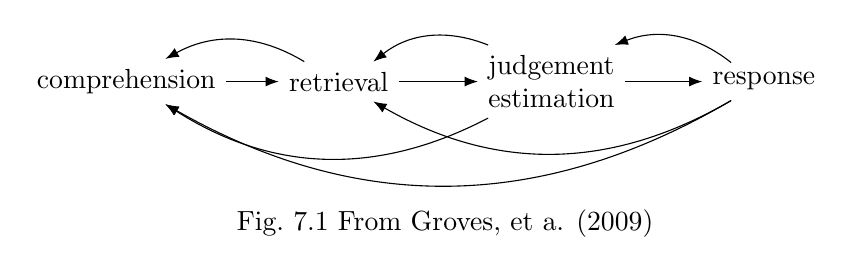
\begin{tikzpicture}[scale=.9]
\usetikzlibrary{arrows.meta}

\node [align=center, thick] (comp)  at (0,0) {comprehension};
\node [align=center, thick] (retr) at (3,0) {retrieval};
\node [align=center, thick] (judg) at (6,0) {judgement\\estimation};
\node [align=center, thick] (resp) at (9,0) {response};

\path [-Latex] (comp) edge (retr) (retr) edge (judg) (judg) edge (resp);
\draw [-Latex] (resp) to [bend right] (judg);
\draw [-Latex] (judg) to [bend right] (retr);
\draw [-Latex] (retr) to [bend right] (comp);
\draw [-Latex] (resp) to [bend left] (retr);
\draw [-Latex] (judg) to [bend left] (comp);
\draw [-Latex] (resp) to [bend left] (comp);

\node [align=center] at (4.5,-2) {Fig.\ 7.1 From Groves, et a. (2009)};

\end{tikzpicture}
\end{center}
\end{frame}

\section{Errors in Answering Questions}

\begin{concept}{comprehension}
a \emph{respondent's} understanding of the question
\end{concept}

\begin{frame}
\begin{description}
\item[Grammar] ambiguity arises from different interpretations of question \pause
\item[Excessive complexity] respondent has difficulty retaining relevant question information in mind to answer question \pause
\item[Faulty presupposition] assumes some state of the world that may not be true \pause
\item[Vague concepts or quantifiers] respondents may differ on meaning of question or response categories \pause
\item[Unfamiliar terms] refers to something that a respondent might not recognize \pause
\item[False inference] respondents try to figure out what a question is ``really'' asking \pause
\end{description}
\end{frame}

\begin{concept}{retrieval}
{the process of recalling information relevant to answering the question from long-term memory, Groves, et al.\ 221}
\end{concept}

\begin{frame}
Retrieval relates to three basic concepts: 
\begin{itemize}
\item Salience of the event 
\item Frequency of event 
\item Elapsed time since the event
\end{itemize}
\end{frame}

\begin{concept}{measurement (error) model}
{a statistical depiction of a process that generates error}
\end{concept}

\begin{frame}
Groves, et al.\ present this \emph{measurement model}:

\[y_i = \mu_i\left(ae^{-bt}\right) + \epsilon_i \]

\begin{description}
\item[$\mu_i$] number of events experienced by the $i$th respondent
\item[$y_i$] report of respondent $i$ to the question
\item[$a$] proportion of events that are reported
\item[$b$] rate of decline in reporting events over time
\end{description}
\end{frame}

\begin{concept}{estimation}
{process of combining or supplementing what the respondent has retrieved}
\end{concept}

\begin{frame}
\textbf{Estimation}\\
People use three strategies to estimate behaviors\\
\begin{minipage}{.75\textwidth}
\begin{description}
\item[Recall \& count] respondent will try to recall all of the times that they engaged in the behavior during the \emph{reference period} and count those events
\item[Rate-based] respondent will create a rate about how often per some unit of time and then multiply that by the \emph{reference period}
\item[Impression-based] respondents will create an impression of how often they do something
\end{description}
\end{minipage}\pause%
\begin{minipage}{.24\textwidth}
\begin{center}

\begin{tikzpicture}
\usetikzlibrary{arrows.meta}
\node [align=center] (least)  at (0,0) {Least effort};
\node [align=center] (most) at (0,4) {Most effort};
\path [-Latex] (least) edge (most);
\end{tikzpicture}
\end{center}
\end{minipage}
\end{frame}

\begin{frame}
Can use a couple different types of responses:
\begin{itemize}
\item Open-ended numeric
\item Closed with ordinal scale (prone to primacy and re\-cen\-cy effects)
\item Closed with categorical scale (prone to primacy and re\-cen\-cy effects)
\end{itemize}
\end{frame}

\begin{concept}{primacy effect}{people tend to benchmark ideas to the first response that they encounter and base judgments on that first option}
\end{concept}

\begin{concept}{recency effect}{people tend to respond more to the \emph{last} response given}
\end{concept} 

\begin{concept}{acquiescence effect}{people tend to like to agree more than they like to disagree}
\end{concept} 

\section{Writing Good Questions}

\begin{frame}{Nonsensitive Behavior Questions}
\begin{enumerate}\small
\item Create comprehensive and mutually exclusive response categories
\item Make question as specific as possible
\item Use familiar words
\item Lengthen questions to add memory cues to improve recall (suggest to respondent what you want them to consider)
\item When forgetting is likely, use aided recall (e.g. use subcategories to questions)\hrule\vspace{.3em}
\item Use a diary
\item Use a life history calendar
\item Ask respondent to use household records to confirm answers
\item Allow a proxy to report for the respondent
\end{enumerate}
\end{frame}

\begin{frame}{Sensitive Behavior Questions}
\begin{enumerate}\small
\item Use open rather than closed questions for eliciting the frequency of sensitive behaviors
\item Use long rather than short questions
\item Use familiar words
\item Deliberately load the question to reduce misreporting (write something that shows that certain behaviors are ``okay'' to reduce motivated misreporting)
\item Ask about long periods before asking about more recent behaviors
\item Embed sensitive question among other sensitive items to make it stand out less
\item Add items to assess the sensitivity of behavioral items
\hrule\vspace{.3em}
\item Allow the respondent to administer the survey to him-\slash herself 
\item Collect data in a diary
\item Collect validation data 
\end{enumerate}
\end{frame}

\begin{frame}{Attitude Questions Pt.\ 1}
\begin{enumerate}
\item<1> Specify the attitude object clearly
\item<1> Measure the strength of the attitude, if necessary using separate items (to avoid double-barreled questions)
\item<1> Use bipolar items except when they might miss key information
\item<1> Carefully consider the alternatives mentioned in the question (they have a big impact on the answers)
\item<1> In measuring change over time or over different groups, ask the same questions
\item<1> When asking both general and specific questions about a topic, ask general items first
\item<1> When asking about multiple items, start with the least popular one
\end{enumerate}
\end{frame}

\begin{frame}{Attitude Questions Pt.\ 2}
\begin{enumerate}
\item<2> Use closed questions for measuring attitudes
\item<2> Use five- or seven-point scales and label every point
\item<2> Start with the end of the scale that is least popular
\item<2> Use analog devices (such as thermometers) to collect more detailed scale information
\item<2> Use ranking only if the respondents can see all alternatives; otherwise use pair-wise comparisons
\item<2> Get ratings for every item of interest; do not use check-all-that-apply items
\end{enumerate}
\end{frame}

\begin{concept}{double-barreled question}{questions that ask about two attitudes simultaneously}
\end{concept}

\begin{frame}
Question from the book on page 249:\\
\textit{Do you favor legalized abortion because it gives women the right to choose?}

\end{frame}

\begin{concept}{bipolar approach}{questions that ask respondents to choose between plausible alternatives}
\end{concept}
\end{document}


